%% -*- coding: utf-8 -*-
\documentclass[12pt,a4paper]{scrartcl} 
\usepackage[utf8]{inputenc}
\usepackage[english,russian]{babel}
\usepackage{indentfirst}
\usepackage{misccorr}
\usepackage{graphicx}
\usepackage{amsmath}
\usepackage{float}

\usepackage{xcolor}
\usepackage{hyperref}
\hypersetup{colorlinks,
  pdftitle={The title of your document},
  pdfauthor={Your name},
  allcolors=[RGB]{000 000 000}}

\begin{document}
\begin{titlepage}
  \begin{center}

    Санкт-Петербургский политехнический университет Петра Великого

    \vspace{0.25cm}
    
    Институт прикладной математики и механики
    
    Кафедра «Прикладная математика»
    \vfill

	\vspace{0.25cm}
	    Отчёт\\
	по лабораторной работе №5\\
	по дисциплине\\
	«Математическая статистика»

  \bigskip

\end{center}
\vfill

\newlength{\ML}
\settowidth{\ML}{«\underline{\hspace{0.7cm}}» \underline{\hspace{2cm}}}
\hfill\begin{minipage}{0.4\textwidth}
  Выполнил студент\\ В.\,А.~Рыженко\\
\end{minipage}%
\bigskip

\hfill\begin{minipage}{0.4\textwidth}
  Проверил:\\
к.ф.-м.н., доцент\\
Баженов Александр Николаевич\\
\end{minipage}%
\vfill

\begin{center}
  Санкт-Петербург, 2020 г.
\end{center}
\end{titlepage}

\tableofcontents
\listoffigures
\listoftables
\newpage

\section{Постановка задачи}
 
Сгенерировать двумерные выборки размерами 20, 60, 100 для нормального двумерного распределения $N(x,y,0,0,1,1, \rho)$.
Коэффициент корреляции $\rho$ взять равным 0, 0.5, 0.9.
Каждая выборка генерируется 1000 раз и для неё вычисляются: среднее значение, среднее значение квадрата и дисперсия коэффициентов
корреляции Пирсона, Спирмена и квадрантного коэффициента корреляции.
Повторить все вычисления для смеси нормальных распределений:
\begin{equation}\label{eq:smes}
\centering
f(x, y) 0.9N(x, y, 0, 0, 1, 1, 0.9) + 0.1N(x, y, 0, 0, 10, 10, -0.9).
\end{equation}

Изобразить сгенерированные точки на плоскости и нарисовать эллипс
равновероятности.

\section{Теория}

\subsection{Двумерное нормальное распределение}
	Двумерная случайная величина (X,Y ) называется распределённой нормально (или просто нормальной), если её плотность вероятности определена формулой
	\begin{equation}
	    N(x, y, \bar{x}, \bar{y}, \sigma_{x}, \sigma_{y}, \rho) = 
	    \frac{1}{2\pi\sigma_{x}\sigma_{y}\sqrt{1-\rho^{2}}} \times
	    exp{\begin{Bmatrix}
	        -\frac{1}{2(1-\rho^{2})}
	        \begin{bmatrix}
	        \frac{(x-\bar{x})^{2}}{\sigma_{x}^{2}} - 2\rho\frac{(x-\bar{x})(y-\bar{y})}{\sigma_{x}\sigma_{y}} + \frac{(y-\bar{y})^{2}}{\sigma_{y}^{2}}
            \end{bmatrix}
            \end{Bmatrix}}
	\end{equation}
	Компоненты X,Y двумерной нормальной случайной величины также распределены нормально с математическими ожиданиями $\bar{x}$,$\bar{y}$ и средними квадратическими отклонениями $\sigma_{x},\sigma_{y}$ соответственно.
	Параметр $\rho$ называется коэффициентом корреляции.


	
	\subsection{Корреляционный момент (ковариация) и коэффициент корреляции}
	Корреляционным моментом, иначе ковариацией, двух случайных величин X и Y называется математическое ожидание произведения отклонений этих случайных величин от их математических ожиданий.
	\begin{equation}
	    K = cov(X, Y) = M[(X - \bar{x})(Y - \bar{y})]
	   \label{K}
	\end{equation}
	Коэффициентом корреляции $\rho$ двух случайных величин X и Y называется отношение их корреляционного момента к произведению их средних квадратических отклонений:
	\begin{equation}
	    \rho = \frac{K}{\sigma_{x}\sigma_{y}}
	    \label{ro}
	\end{equation}
	Коэффициент корреляции — это нормированная числовая характеристика, являющаяся мерой близости зависимости между случайными величинами к линейной.

	\subsection{Выборочные коэффициенты корреляции}
	\subsubsection{Выборочный коэффициент корреляции Пирсона}
	Пусть по выборке значений ${x_{i},y_{i}}^{n}_{1}$ двумерной с.в. (X,Y ) требуется оценить коэффициент корреляции $\rho = \frac{cov(X,Y)}{\sqrt{DXDY}}$ . Естественной оценкой для $\rho$ служит его статистический аналог в виде выборочного коэффициента корреляции, предложенного К.Пирсоном, —
	\begin{equation}
	    r = \frac{
	    \frac{1}{n}\sum{(x_{i} - \bar{x})(y_{i}-\bar{y})}
	    }{
	    \sqrt{\frac{1}{n}\sum{(x_{i} - \bar{x})^{2}}\frac{1}{n}\sum{(y_{i} - \bar{y})^{2}}}
	    }=\frac{K}{s_{X}s_{Y}},
	    \label{r}
	\end{equation}
	где $K,s^{2}_{X},s^{2}_{Y}$ — выборочные ковариация и дисперсии с.в. X и Y.


    \subsubsection{Выборочный квадрантный коэффициент корреляции}
    Кроме выборочного коэффициента корреляции Пирсона, существуют и другие оценки степени взаимосвязи между случайными величинами. К ним относится выборочный квадрантный коэффициент корреляции
    \begin{equation}
        r_{Q} = \frac{(n_{1} + n_{3}) - (n_{2} + n_{4})}{n},
        \label{rQ}
    \end{equation}
    где $n_{1}, n_{2},n_{3}$ и $n_{4}$ — количества точке с координатами $(x_{i},y_{i})$, попавшими соответственно в I, II, III и IV квадранты декартовой системы с осями $x' = x-med x, y' = y- med y $ и с центром в точке с координатами (med x,med y).


	  
	\subsubsection{Выборочный коэффициент ранговой корреляции Спирмена}
    На практике нередко требуется оценить степень взаимодействия между качественными признаками изучаемого объекта. Качественным называется признак, который нельзя измерить точно, но который позволяет сравнивать изучаемые объекты между собой и располагать их в порядке убывания или возрастания их качества. Для этого объекты выстраиваются в определённом порядке в соответствии с рассматриваемым признаком. Процесс упорядочения называется ранжированием, и каждому члену упорядоченной последовательности объектов присваивается ранг, или порядковый номер. Например, объекту с наименьшим значением признака присваивается ранг 1, следующему за ним объекту — ранг 2, и т.д. Таким образом, происходит сравнение каждого объекта со всеми объектами изучаемой выборки.
    \newline
    Если объект обладает не одним, а двумя качественными признаками — переменными X и Y , то для исследования их взаимосвязи используют выборочный коэффициент корреляции между двумя последовательностями рангов этих признаков.
    \newline
    Обозначим ранги, соотвествующие значениям переменной X, через u, а ранги, соотвествующие значениям переменной Y, — через v.
    \newline
    Выборочный коэффициент ранговой корреляции Спирмена определяется как выборочный коэффициент корреляции Пирсона между рангами u,v переменных X,Y :
    \begin{equation}
         r_{S} = \frac{
	    \frac{1}{n}\sum{(u_{i} - \bar{u})(v_{i}-\bar{v})}
	    }{
	    \sqrt{\frac{1}{n}\sum{(u_{i} - \bar{u})^{2}}\frac{1}{n}\sum{(v_{i} - \bar{v})^{2}}}
	    },
	    \label{rS}
    \end{equation}
    где $\bar{u} = \bar{v} = \frac{1 + 2 + ... + n}{n} = \frac{n + 1}{2}$ — среднее значение рангов.

	
	\subsection{Эллипсы рассеивания}
	Рассмотрим поверхность распределения, изображающую функцию (1). Она имеет вид холма, вершина которого находится над точкой $(\bar{x},\bar{y})$.
	\newline
    В сечении поверхности распределения плоскостями, параллельными оси $ N(x, y, \bar{x}, \bar{y}, \sigma_{x}, \sigma_{y}, \rho)$, получаются кривые, подобные нормальным кривым распределения. В сечении поверхности распределения плоскостями, параллельными плоскости xOy, получаются эллипсы. Напишем уравнение проекции такого эллипса на плоскость xOy: 
    \begin{equation}
        \frac{(x-\bar{x})^{2}}{\sigma_{x}^{2}} - 
        2\rho\frac{(x-\bar{x})(y-\bar{y})}{\sigma_{x}\sigma_{y}}+
        \frac{(y-\bar{y})^{2}}{\sigma_{y}^{2}} = const
        \label{ellipse}
    \end{equation}
    Уравнение эллипса (8) можно проанализировать обычными методами аналитической геометрии. Применяя их, убеждаемся, что центр эллипса (8) находится в точке с координатами $(\bar{x},\bar{y})$; что касается направления осей симметрии эллипса, то они составляют с осью Ox углы, определяемые уравнением
    \begin{equation}
        \tg(2\alpha) = \frac{2\rho\sigma_{x}\sigma_{y}}{\sigma_{x}^{2} - \sigma_{y}^{2}}
        \label{angle}
    \end{equation}
    Это уравнение дает два значения углов: $\alpha$ и $\alpha_{1}$, различающиеся на $\frac{\pi}{2}$.
    \newline
    Таким образом, ориентация эллипса (8) относительно координатных осей находится в прямой зависимости от коэффициента корреляции $\rho$ системы (X,Y); если величины не коррелированны (т.е. в данном случае и независимы), то оси симметрии эллипса параллельны координатным осям; в противном случае они составляют с координатными осями некоторый угол.
    \newline
    Пересекая поверхность распределения плоскостями, параллельными плоскости xOy, и проектируя сечения на плоскость xOy мы получим целое семейство подобных и одинаково расположенных эллипсов с общим центром $(\bar{x},\bar{y})$. Во всех точках каждого из таких эллипсов плотность распределения $ N(x, y, \bar{x}, \bar{y}, \sigma_{x}, \sigma_{y}, \rho)$ постоянна. Поэтому такие эллипсы называются эллипсами равной плотности или, короче эллипсами рассеивания. Общие оси всех эллипсов рассеивания называются главными осями рассеивания

\section {Реализация}
Лабораторная работа выполнена с помощью встроенных средств языка программирования Python в среде разработки Visual Code. Исходный код лабораторной работы приведён в приложении.
 
\section{Результаты}

\subsection{Выборочные коэффициенты корреляции}

\begin{table}[H]
    \centering
    \begin{tabular}{| c | c | c | c |}
\hline
 $\rho$= 0.1 & r       & $r_S$   & $r_Q$   \\ \hline
 $E(z)$      & 0.09583 & 0.0881  & 0.0618  \\ \hline
 $E(z^2)$    & 0.06164 & 0.06158 & 0.05472 \\ \hline
 $D(z)$      & 0.05246 & 0.05382 & 0.0509  \\ \hline
&  & & \\  \hline
 $\rho$= 0.5 & r       & $r_S$   & $r_Q$   \\ \hline
 $E(z)$      & 0.48972 & 0.46149 & 0.3333  \\ \hline
 $E(z^2)$    & 0.27144 & 0.24917 & 0.15597 \\ \hline
 $D(z)$      & 0.03161 & 0.0362  & 0.04488 \\ \hline
&  & & \\  \hline
 $\rho$= 0.9 & r       & $r_S$   & $r_Q$   \\ \hline
 $E(z)$      & 0.89417 & 0.86592 & 0.7107  \\ \hline
 $E(z^2)$    & 0.80188 & 0.75436 & 0.53101 \\ \hline
 $D(z)$      & 0.00234 & 0.00454 & 0.02592 \\
\hline
\end{tabular}
 \caption{Двумерное нормальное распределение, n = 20}
\label{tab:norm_20}
\end{table}

\begin{table}[H]
\centering
\begin{tabular}{| c | c | c | c |}
\hline
 $\rho$= 0.1 & r       & $r_S$   & $r_Q$   \\ \hline
 $E(z)$      & 0.09635 & 0.09191 & 0.0616  \\ \hline
 $E(z^2)$    & 0.0261  & 0.02536 & 0.02056 \\ \hline
 $D(z)$      & 0.01681 & 0.01692 & 0.01677 \\ \hline
&  & & \\  \hline
 $\rho$= 0.5 & r       & $r_S$   & $r_Q$   \\ \hline
 $E(z)$      & 0.49818 & 0.47721 & 0.33587 \\ \hline
 $E(z^2)$    & 0.25849 & 0.23911 & 0.12774 \\ \hline
 $D(z)$      & 0.01031 & 0.01138 & 0.01493 \\ \hline
&  & & \\  \hline
 $\rho$= 0.9 & r       & $r_S$   & $r_Q$   \\ \hline
 $E(z)$      & 0.89831 & 0.88219 & 0.7134  \\ \hline
 $E(z^2)$    & 0.80768 & 0.77943 & 0.51793 \\ \hline
 $D(z)$      & 0.00072 & 0.00118 & 0.00899 \\
\hline
\end{tabular}
 \caption{Двумерное нормальное распределение, n = 60}
\label{tab:norm_60}
\end{table}

\begin{table}[H]
\centering
\begin{tabular}{| c | c | c | c |}
\hline
 $\rho$= 0.1 & r       & $r_S$   & $r_Q$   \\ \hline
 $E(z)$      & 0.09685 & 0.09097 & 0.0623  \\ \hline
 $E(z^2)$    & 0.01949 & 0.01842 & 0.01368 \\ \hline
 $D(z)$      & 0.01011 & 0.01015 & 0.0098  \\ \hline
&  & & \\  \hline
 $\rho$= 0.5 & r       & $r_S$   & $r_Q$   \\ \hline
 $E(z)$      & 0.49763 & 0.47816 & 0.3355  \\ \hline
 $E(z^2)$    & 0.25309 & 0.23481 & 0.12132 \\ \hline
 $D(z)$      & 0.00546 & 0.00617 & 0.00876 \\ \hline
&  & & \\  \hline
 $\rho$= 0.9 & r       & $r_S$   & $r_Q$   \\ \hline
 $E(z)$      & 0.89931 & 0.88653 & 0.71348 \\ \hline
 $E(z^2)$    & 0.80912 & 0.78653 & 0.5139  \\ \hline
 $D(z)$      & 0.00036 & 0.0006  & 0.00485 \\
\hline
\end{tabular}
 \caption{Двумерное нормальное распределение, n = 100}
\label{tab:norm_100}
\end{table}

\begin{table}[H]
\centering
\begin{tabular}{| c | c | c | c |}
\hline
 n= 20    & r       & $r_S$   & $r_Q$   \\ \hline
 $E(z)$   & 0.7856  & 0.74974 & 0.589   \\ \hline
 $E(z^2)$ & 0.62594 & 0.57467 & 0.3803  \\ \hline
 $D(z)$   & 0.00877 & 0.01255 & 0.03338 \\ \hline
&  & & \\  \hline
 n= 60    & r       & $r_S$   & $r_Q$   \\ \hline
 $E(z)$   & 0.7889  & 0.7685  & 0.58197 \\ \hline
 $E(z^2)$ & 0.62474 & 0.59391 & 0.34904 \\ \hline
 $D(z)$   & 0.00238 & 0.00332 & 0.01035 \\ \hline
&  & & \\  \hline
 n= 100   & r       & $r_S$   & $r_Q$   \\ \hline
 $E(z)$   & 0.79138 & 0.77284 & 0.58436 \\ \hline
 $E(z^2)$ & 0.62771 & 0.59925 & 0.348   \\ \hline
 $D(z)$   & 0.00143 & 0.00197 & 0.00652 \\
\hline
\end{tabular}
 \caption{Смесь нормальных распределений}
\label{tab:mix}
\end{table}

\subsection{Эллипсы рассеивания}
	
	\begin{figure}[H]
	    \centering
	    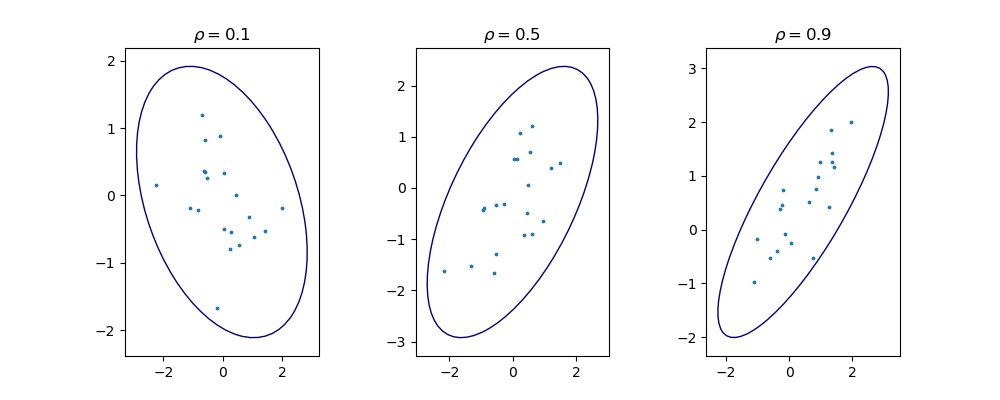
\includegraphics[width=1\textwidth]{n=20.png}
	    \caption{ Двумерное нормальное распределение, n = 20}
	    \label{fig:f20}
	\end{figure}
	
	\begin{figure}[H]
	    \centering
	    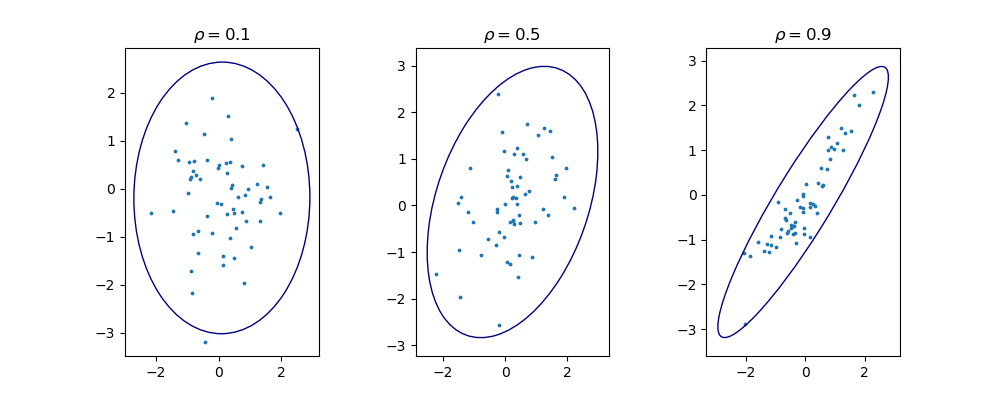
\includegraphics[width=1\textwidth]{n=60.png}
	    \caption{Двумерное нормальное распределение, n = 60}
	    \label{fig:f60}
	\end{figure}
	
	\begin{figure}[H]
	    \centering
	    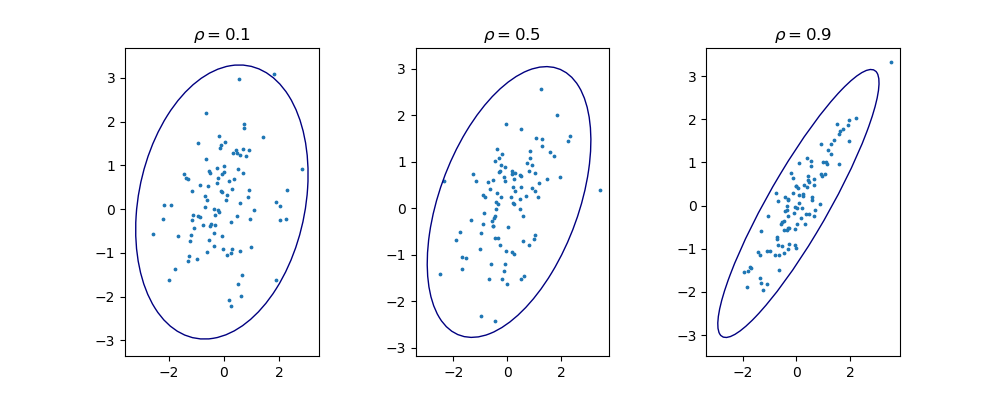
\includegraphics[width=1\textwidth]{n=100.png}
	    \caption{Двумерное нормальное распределение, n = 100}
	    \label{fig:f100}
	\end{figure}

\section{Обсуждение}
Для двумерного нормального распределения дисперсии выборочных коэффициентов корреляции упорядочены следующим образом: $r < r_{S} < r_{Q}$; для смеси распределений: $r_{Q} < r_{S} < r$.
\newline
Процент попавших элементов выборки в эллипс рассеивания (95$\%$-ная доверительная область) примерно равен его теоретическому значению (95$\%$).

\section{Приложения}
Репозиторий на GitHub с релизацией: \href{https://github.com/WiillyWonka/MatStat}{github.com}.
\end{document}
